\chapter*{Иллюстрации к правобережью}
\addcontentsline{toc}{chapter}{Иллюстрации к правобережью}


\begin{center}
\includegraphics[width=\linewidth]{rpix/IMG_20130826_173208.jpg}

\textit{Арсенальский дом, 2013 год.}
\end{center}

\newpage

\vspace*{\fill}
\begin{center}
\includegraphics[width=\linewidth]{rpix/bayk.jpg}

\textit{Байкова гора до революции, поселение рядом с кладбищем.}
\end{center}
\vspace*{\fill}
\newpage


\begin{center}
\includegraphics[width=0.95\linewidth]{rpix/IMG_3949.JPG}

\textit{Беличи, остатки юго-западной части села, ныне «13-й микрорайон Беличи».}
\end{center}


\begin{center}
\includegraphics[width=\linewidth]{rpix/IMG_3964.JPG}

\textit{Беличи, почти там же.}
\end{center}


\newpage


\begin{center}
\includegraphics[width=\linewidth]{rpix/belor-14.jpg}

\textit{Расположенная в овраге Белорусская улица, слева видны трамвайные рельсы. По дну оврага раньше протекал ручей Скоморох, ныне заточенный в коллектор.}
\end{center}


\begin{center}
\includegraphics[width=\linewidth]{rpix/bolnikolay.jpg}

\textit{Большой Николай, колокольня.}
\end{center}



\begin{center}
\includegraphics[width=\linewidth]{rpix/IMG_20190619_125950.jpg}

\textit{Окрестности источника Бусловки.}
\end{center}


\begin{center}
\includegraphics[width=\linewidth]{rpix/IMG_20190619_125951.jpg}

\textit{Окрестности источника Бусловки.}
\end{center}


\newpage


\begin{center}
\includegraphics[width=\linewidth]{rpix/1973.jpg}

\textit{Глинка, озеро в 1971 году. Снимок Войтеха Туржанского. Слева – Черная гора, на заднем плане, за кирпичным заводом, на другой горе (за Лыбедью) – Саперная слободка.}
\end{center}

\newpage


\begin{center}
\includegraphics[width=\linewidth]{rpix/imag0025.jpg}

\textit{Глинка, 2005 год. Вид на хрущовки над озером.}
\end{center}



\begin{center}
\includegraphics[width=\linewidth]{rpix/gonch.jpg}

\textit{Гончары, вид на Гончаровскую улицу. Конечно же, дореволюционная открытка.}
\end{center}


\newpage


\begin{center}
\includegraphics[width=\linewidth]{rpix/gorka.jpg}

\textit{Горка, 2003 год.}
\end{center}

\begin{center}
\includegraphics[width=\linewidth]{rpix/IMG_20130826_143424.jpg}

\textit{Горка, 2013 год.}
\end{center}


\newpage
\vspace*{\fill}
\begin{center}
\includegraphics[width=\linewidth]{rpix/IMG_20130826_143421.jpg}

\textit{Горка, 2013 год, вид чуть левее. За серым гаражом – осколок частного сектора в несколько домов, с узеньким переулком между дворами.}
\end{center}
\vspace*{\fill}

\newpage
\vspace*{\fill}

\begin{center}
\includegraphics[width=\linewidth]{rpix/domrich.jpg}

\textit{Дом Ричарда, дореволюционная открытка. За ним видно гору Киселевку с кирпичной кладбищенской стеной – там было кладбище Флоровского монастыря, разоренные остатки коего, равно как и стену, можно посетить и в наши дни.}
\end{center}
\vspace*{\fill}


\newpage

\begin{center}
\includegraphics[width=\linewidth]{rpix/IMG_1401.JPG}

\textit{Жаба. Вход.}
\end{center}


\begin{center}
\includegraphics[width=\linewidth]{rpix/IMG_1402.JPG}

\textit{Жаба. Эстрада.}
\end{center}

\newpage

\vspace*{\fill}


\begin{center}
\includegraphics[width=\linewidth]{rpix/kamenka.jpg}
\textit{Каменка и Рогостинка на карте 1746 года.}
\end{center}


\begin{center}
\includegraphics[width=\linewidth]{rpix/IMG_20150504_142738.jpg}
\textit{Каменка у истока, 2015.}
\end{center}

\vspace*{\fill}



\begin{center}
\includegraphics[width=\linewidth]{rpix/IMG_20170611_150523.jpg}
\textit{Кинь-грусть, 2017.}
\end{center}


\begin{center}
\includegraphics[width=\linewidth]{rpix/IMG_20160330_153049.jpg}
\textit{Кирилловские высоты, Иорданское кладбище.}
\end{center}



\vspace*{\fill}

\begin{center}
\includegraphics[width=\linewidth]{rpix/alb.jpg}

\textit{Клов, слева Александровская больница, эти корпуса ныне снесены, примыкали к ул. Мечникова. Наверху на заднем плане – Северная полубашня Киевская крепости, на ул. Госпитальной, существует поныне, но из-за застройки и проложенного бульвара Леси Украинки ее с этой точки больше не видно.}
\end{center}
\vspace*{\fill}

\newpage

\vspace*{\fill}
\begin{center}
\includegraphics[width=\linewidth]{rpix/klov02.jpg}

\textit{Клов, вернее, вид на него как раз с пригорка, где у нас за спиной упомянутая полубашня.}
\end{center}
\vspace*{\fill}

\newpage
\vspace*{\fill}


\begin{center}
\includegraphics[width=\linewidth]{rpix/klov03.jpg}

\textit{Клов, 1914 год – вид из центра города на Клов. Это над ним виднеется Лаврская колокольня, хотя она много дальше. Широкая грунтовая дорога, что взбирается от Клова направо на гору, к Северной полубашне – нынешняя улица Госпитальная. Это сбивает с толку, потому что на первый взгляд думаешь – прообраз бульвара Леси Украинки, а ведь он в наше время левее.}
\end{center}
\vspace*{\fill}

\newpage
\vspace*{\fill}
\begin{center}
\includegraphics[width=\linewidth]{rpix/klov-esp.jpg}

\textit{Кловица течет за забором посередине кадра. Вид на пересечение Эспланадной и Скаскаганского. Конец 19 века.}
\end{center}
\vspace*{\fill}

\newpage


\begin{center}
\includegraphics[width=0.93\linewidth]{rpix/25-04-07_1552.jpg}

\textit{Клов застраивается. 2007. Бульвар Леси Украинки.}
\end{center}


\begin{center}
\includegraphics[width=0.93\linewidth]{rpix/25-04-07_1554.jpg}

\textit{Клов застраивается. 2007. Наверху бульвар Леси.}
\end{center}

\newpage


\begin{center}
\includegraphics[width=0.93\linewidth]{rpix/25-04-07_1554.jpg}

\textit{Клов застраивается. 2007. Наверху бульвар Леси.}
\end{center}

\begin{center}
\includegraphics[width=\linewidth]{rpix/25-04-07_1553.jpg}

\textit{Клов, а тут давно застроено. 2007.}
\end{center}


\newpage
\vspace*{\fill}


\begin{center}
\includegraphics[width=\linewidth]{rpix/IMG_20190504_133527.jpg}

\textit{Клов, 2019. Устье.}
\end{center}

\begin{center}
\includegraphics[width=\linewidth]{rpix/IMG_20190504_133538.jpg}

\textit{Клов, 2019. Устье.}
\end{center}

\vspace*{\fill}


%\begin{center}
%\includegraphics[width=\linewidth]{rpix/25-04-07_1553.jpg}

%\textit{Клов, а тут давно застроено. 2007.}
%\end{center}


%\begin{center}
%\includegraphics[width=\linewidth]{rpix/IMG_20170611_145933.jpg}

%\textit{Княжая гора, 2017.}
%\end{center}

\newpage
\vspace*{\fill}

\begin{center}
\includegraphics[width=\linewidth]{rpix/IMG_20190504_133643.jpg}

\textit{Клов, 2019. Устье прежнего коллектора.}
\end{center}


\begin{center}
\includegraphics[width=\linewidth]{rpix/IMG_20190504_133659.jpg}

\textit{Клов, 2019. Урочище Пятничный Клов, место пятничной тусовки диггеров.}
\end{center}

\vspace*{\fill}

%\begin{center}

%\includegraphics[width=\linewidth]{rpix/IMG_20170611_150002.jpg}

%\textit{Княжая гора, 2017.}
%\end{center}


\newpage

\begin{center}
\includegraphics[width=\linewidth]{rpix/IMG_20170611_145933.jpg}

\textit{Княжая гора, 2017.}
\end{center}



\begin{center}
\includegraphics[width=\linewidth]{rpix/koz-bol.jpg}

\textit{Козье болото (зеленые насаждения в левой серединной части кадра)}
\end{center}



\newpage


\vspace*{\fill}

\begin{center}
\includegraphics[width=\linewidth]{rpix/IMG_20200815_143315.jpg}

\textit{Красный дом, 2020.}
\end{center}


\vspace*{\fill}

\newpage

\begin{center}
\includegraphics[width=\linewidth]{rpix/IMG_20170411_145319.jpg}

\textit{Костопальня, 2017.}
\end{center}


%\begin{center}
%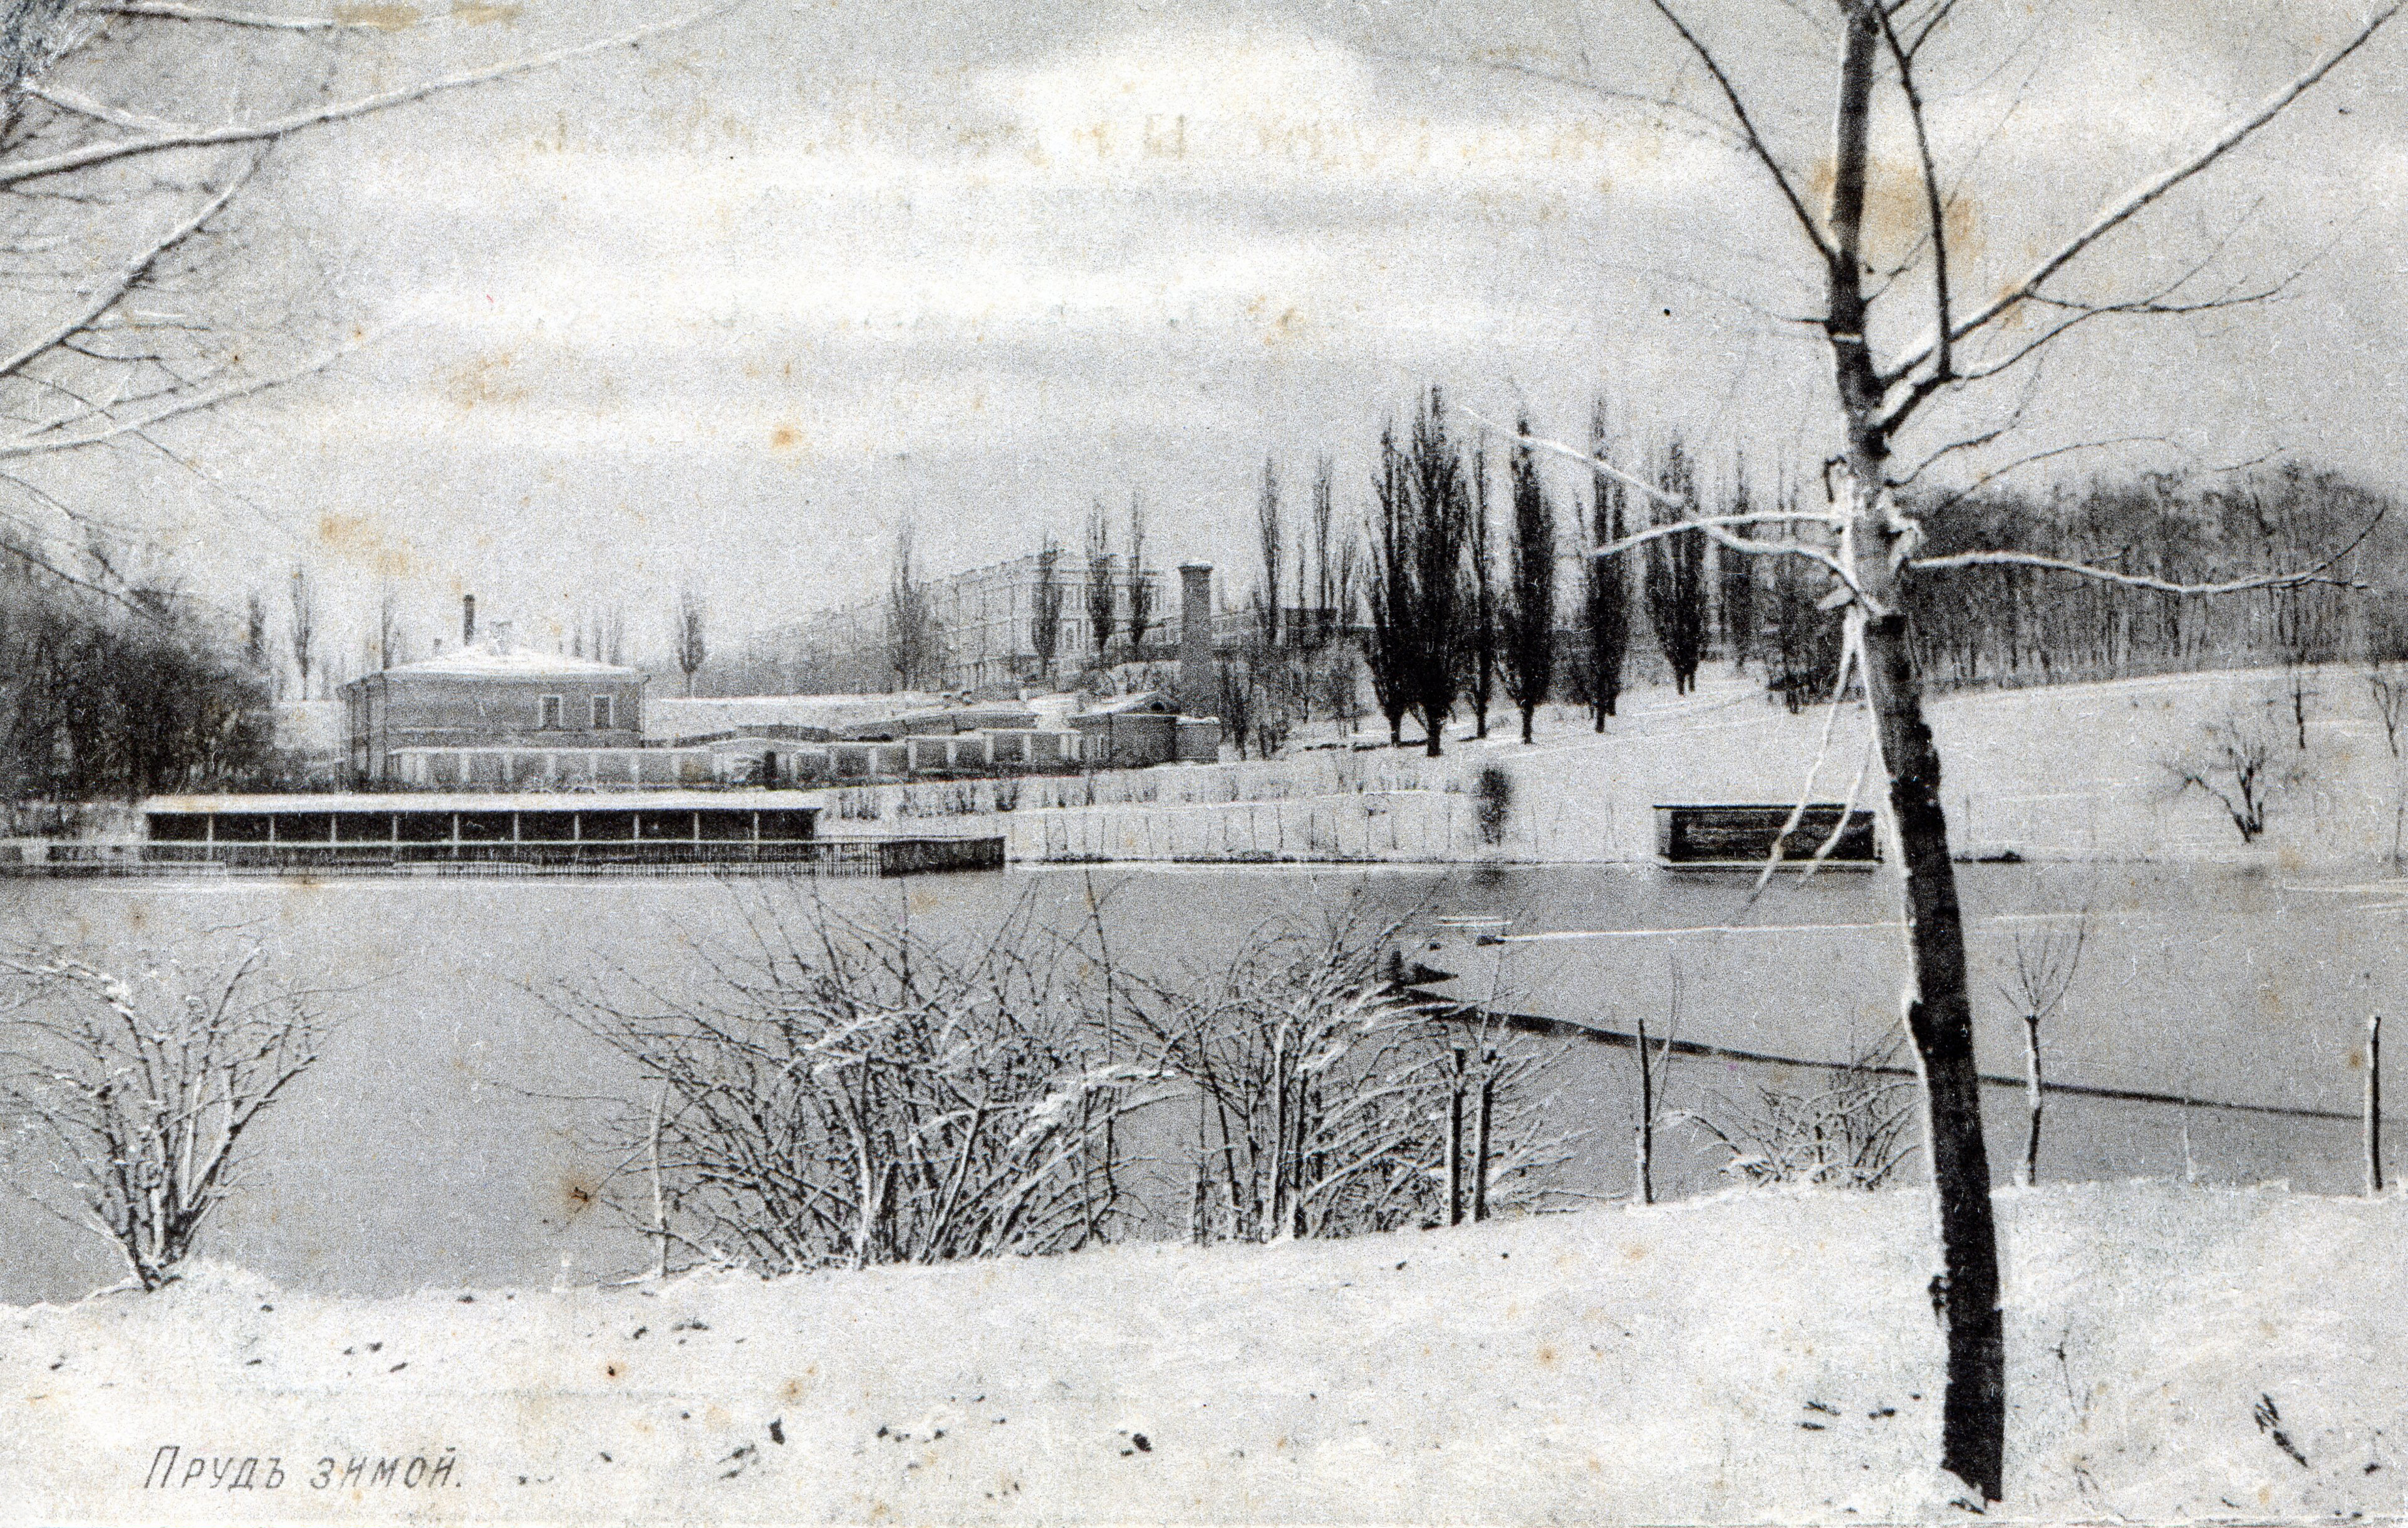
\includegraphics[width=\linewidth]{rpix/lybed-prud-ninjiy-kadet-rosh.jpg}

%\textit{Пруд на Лыбеди.}
%\end{center}


%\begin{center}
%\includegraphics[width=\linewidth]{rpix/%lyb.png}

%\textit{Лыбедь или Киянка?}
%\end{center}

%\begin{center}
%\includegraphics[width=0.95\linewidth]{rpix/%IMG_20191126_132325.jpg}

%\textit{Лыбедь, короткий отрезок старого природного русла.}
%\end{center}

\begin{center}
\includegraphics[width=0.95\linewidth]{rpix/IMG_20190616_135257.jpg}

\textit{Лыбедь вытекает из коллектора у Лысой горы.}
\end{center}


\begin{center}
\includegraphics[width=0.92\linewidth]{rpix/IMG_20191126_132719.jpg}

\textit{Лыбедь течет по рукотворному руслу к устью.}
\end{center}


\begin{center}
\includegraphics[width=0.92\linewidth]{rpix/IMG_20191126_143542.jpg}

\textit{Лыбедь течет по рукотворному руслу к устью.}
\end{center}


\begin{center}
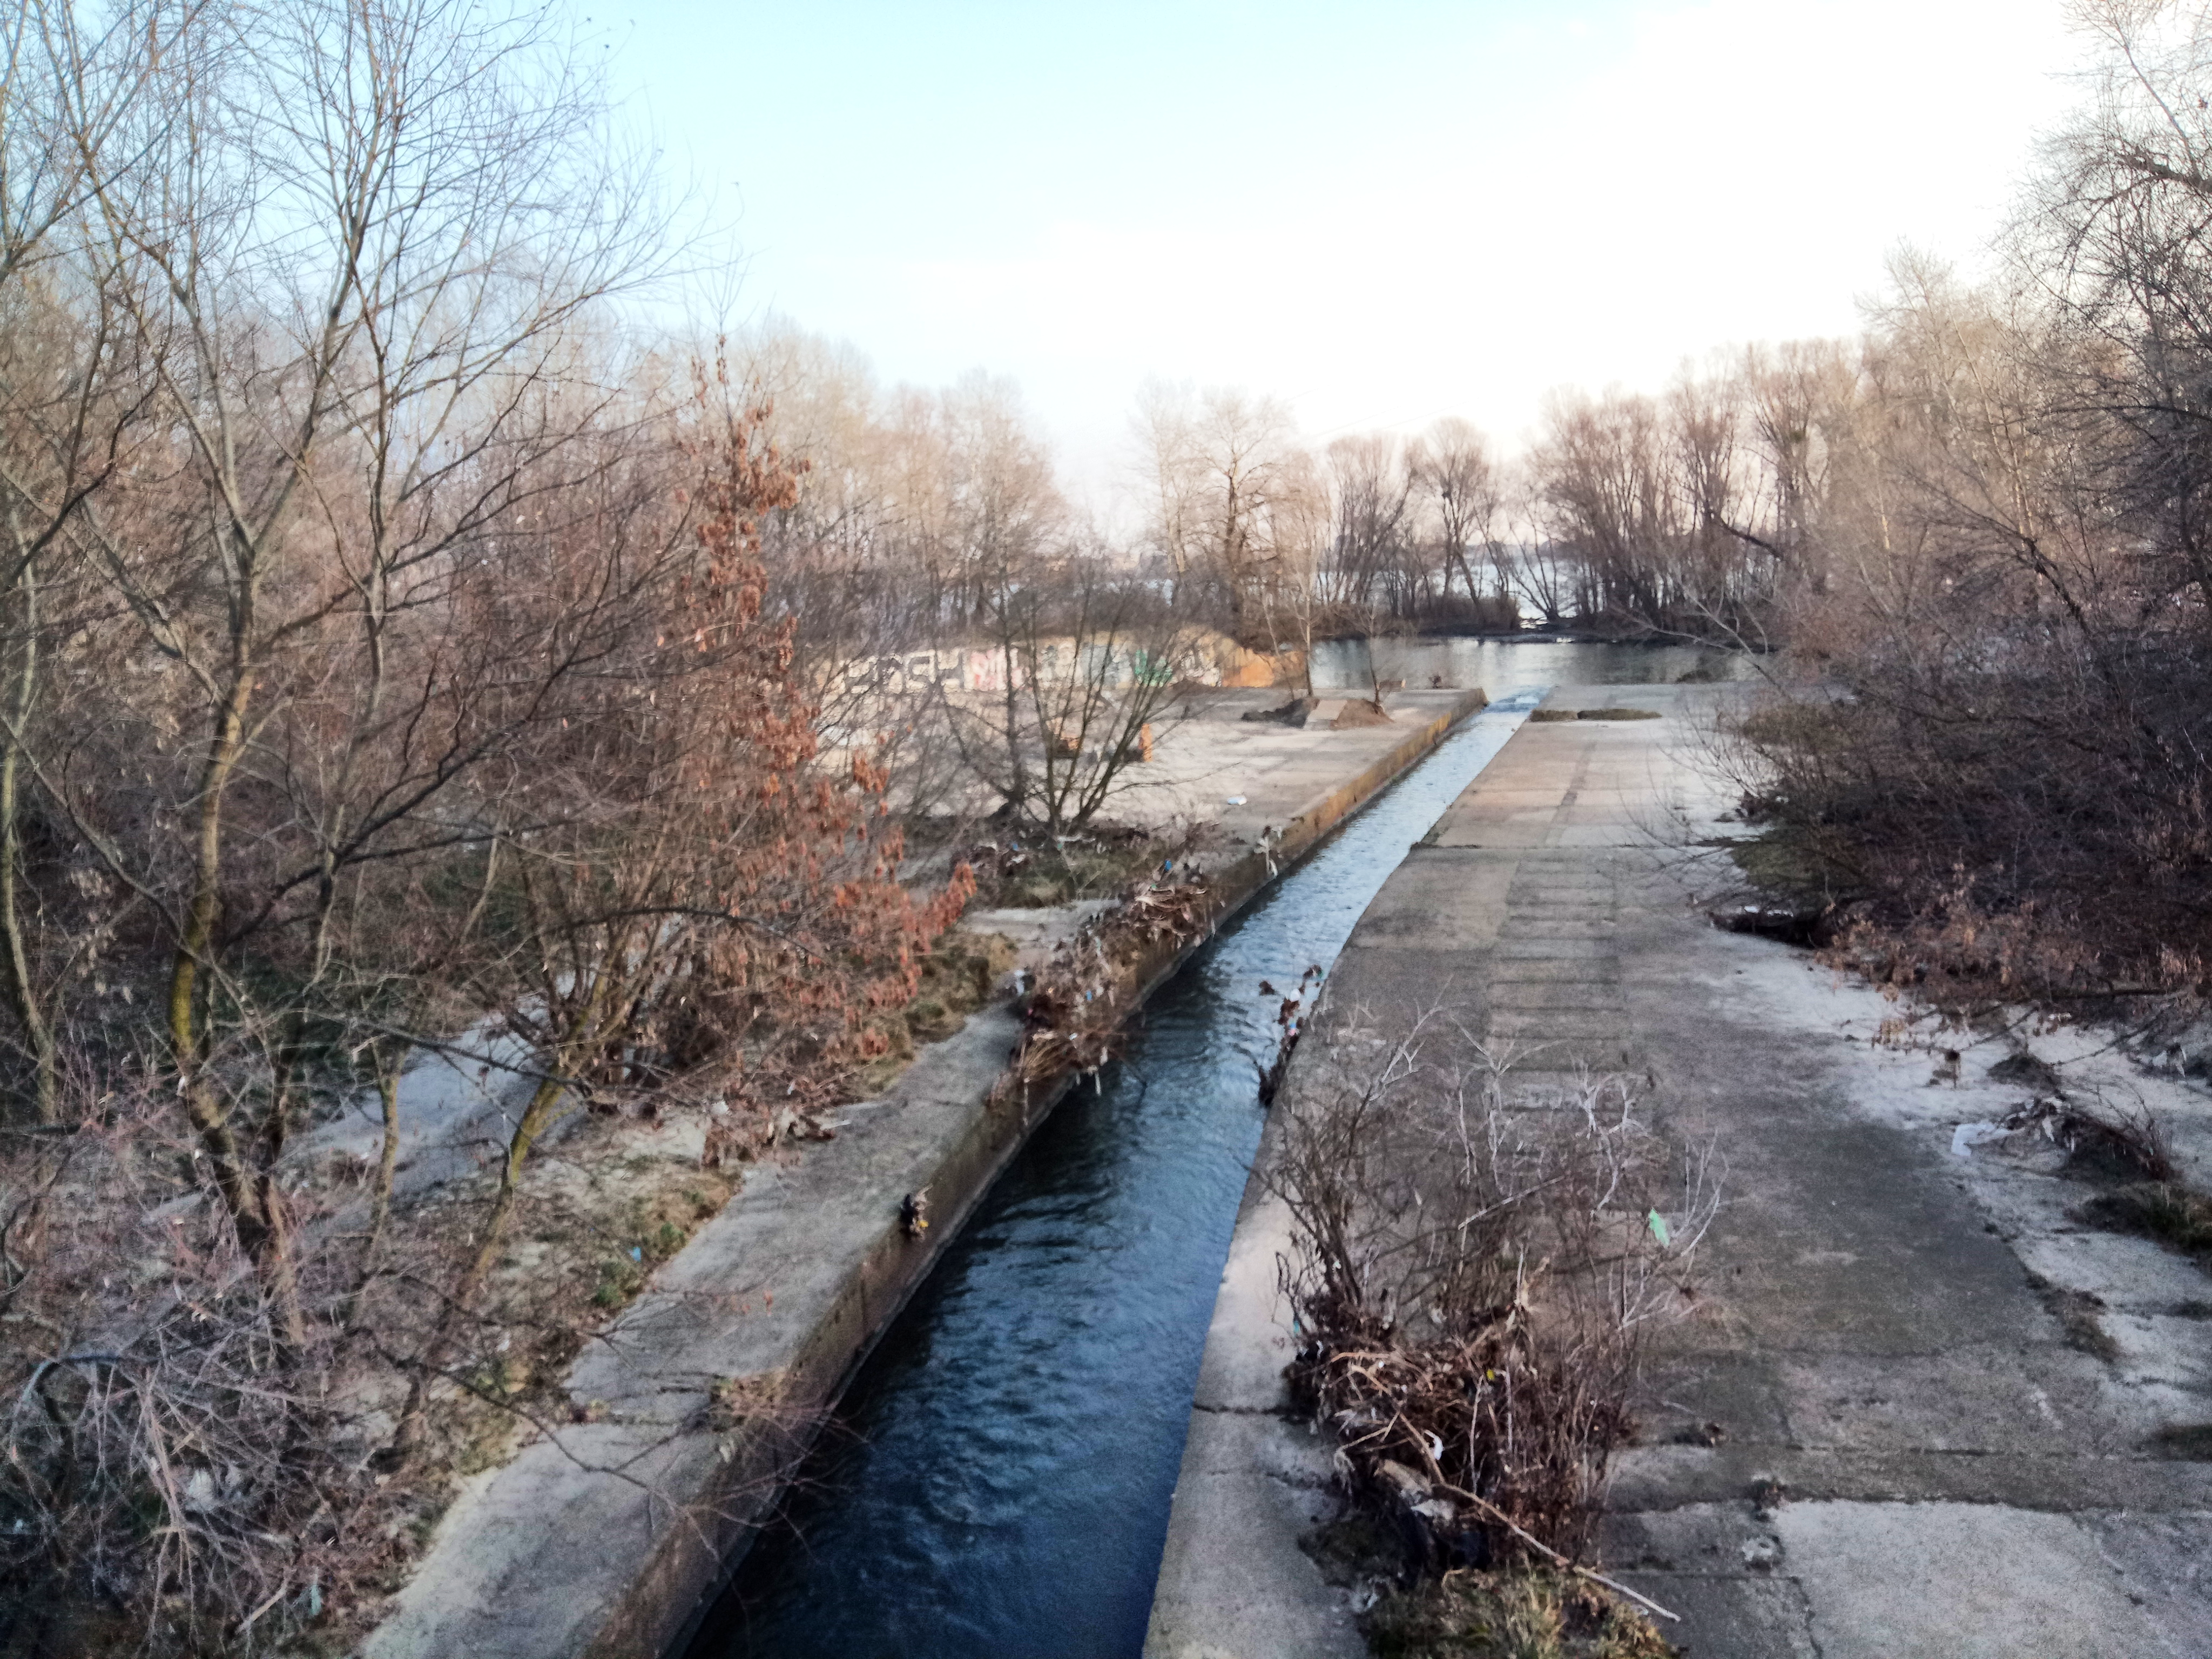
\includegraphics[width=\linewidth]{rpix/IMG_20191126_141033_DRO.jpg}

\textit{Лыбедь, вид на устье.}
\end{center}


\begin{center}
\includegraphics[width=\linewidth]{rpix/IMG_20191126_141702_DRO.jpg}

\textit{Лыбедь, устье.}
\end{center}


\begin{center}
\includegraphics[width=\linewidth]{rpix/IMG_20191126_142103_DRO.jpg}

\textit{Лыбедь, устье.}
\end{center}


\begin{center}
\includegraphics[width=0.95\linewidth]{rpix/IMG_20170402_144928.jpg}

\textit{Монтажник, 2017.}
\end{center}



\begin{center}
\includegraphics[width=0.95\linewidth]{rpix/navod.jpg}

\textit{Наводницкий ручей. 1951, Компаниец-Киянченко Н. Д.}
\end{center}


\begin{center}
\includegraphics[width=\linewidth]{rpix/IMG_20150701_144629.jpg}

\textit{Наводничи, 2015.}
\end{center}


\begin{center}
\includegraphics[width=0.93\linewidth]{rpix/IMG_3981.JPG}

\textit{Нивка, речка, около пруда номер 15 (по ул. Ушакова и Наумовича).}
\end{center}

\begin{center}
\includegraphics[width=0.93\linewidth]{rpix/IMG_3997.JPG}

\textit{Нивка, речка, пруд номер 14 (по ул. Живописной и Верховинной).}
\end{center}


\begin{center}
\includegraphics[width=\linewidth]{rpix/IMG_4375.jpg}

\textit{Никольский старый ввоз.}
\end{center}



\begin{center}
\includegraphics[width=\linewidth]{rpix/IMG_20201109_125203.jpg}

\textit{Ореховатка. Устье. 2020}
\end{center}


\begin{center}
\includegraphics[width=\linewidth]{rpix/IMG_20201109_125811.jpg}

\textit{Ореховатка. Устье. 2020}
\end{center}




\begin{center}
\includegraphics[width=\linewidth]{rpix/pechbaz.jpg}

\textit{Печерский базар, 1912 год.}
\end{center}


\begin{center}
\includegraphics[width=\linewidth]{rpix/IMG_20201109_125816.jpg}

\textit{Пещера Белых сталактитов, вход. 2020.}
\end{center}




\begin{center}
\includegraphics[width=\linewidth]{rpix/IMG_20190504_141816.jpg}

\textit{Протасов яр, 2019. Наверху, вид на Соломенку.}
\end{center}


\begin{center}
\includegraphics[width=\linewidth]{rpix/IMG_20190504_141817.jpg}

\textit{Протасов яр, 2019. На горе, вид на верховье яра.}
\end{center}


\begin{center}
\includegraphics[width=0.90\linewidth]{rpix/DSC_0022.JPG}

\textit{Пятачок, 2007 год. Вид в сторону Бастионной.}
\end{center}


\begin{center}
\includegraphics[width=0.90\linewidth]{rpix/DSC_0021.JPG}

\textit{Пятачок, 2007 год. Вид в сторону Бастионной и «Дары Ланив».}
\end{center}



\begin{center}
\includegraphics[width=0.95\linewidth]{rpix/IMG_20130826_173616.jpg}

\textit{Пятачок, во дворах, 2013 год.}
\end{center}



\begin{center}
\includegraphics[width=\linewidth]{rpix/repyar.jpg}

\textit{Репяхов яр с проложенным по нему Кирилловским спуском. Далее спуск был переименован во Врубелевский и практически исчез.}
\end{center}


\begin{center}
\includegraphics[width=\linewidth]{rpix/repyar1908.jpg}

\textit{Репяхов яр, 1908 год.}
\end{center}


\begin{center}
\includegraphics[width=\linewidth]{rpix/IMG_4332.JPG}

\textit{Рогостинка, 2015.}
\end{center}


\begin{center}
\includegraphics[width=0.95\linewidth]{rpix/imag0041.jpg}

\textit{Собачка, 2005. Наверху, вид на забор ботсада.}
\end{center}


\begin{center}
\includegraphics[width=0.95\linewidth]{rpix/imag0044.jpg}

\textit{Собачка, 2005. Верхняя тропа вдоль забора ботсада.}
\end{center}


\begin{center}
\includegraphics[width=\linewidth]{rpix/imag0052.jpg}

\textit{Собачка, 2005. Остатки спортплощадки.}
\end{center}



\begin{center}
\includegraphics[width=\linewidth]{rpix/IMG_4319.jpg}

\textit{Сырец.}
\end{center}


\begin{center}
\includegraphics[width=\linewidth]{rpix/DSC_0016.JPG}

\textit{«Темп», бывший, конечно. Фото 2007 года.}
\end{center}



\begin{center}
\includegraphics[width=\linewidth]{rpix/IMG_20210601_134915.jpg}

\textit{Тропа Хо Ши Мина. 2021.}
\end{center}



\begin{center}
\includegraphics[width=\linewidth]{rpix/IMG_20210601_134927.jpg}

\textit{Тропа Хо Ши Мина. 2021.}
\end{center}



\begin{center}
\includegraphics[width=\linewidth]{rpix/IMG_20210601_134940.jpg}

\textit{Тропа Хо Ши Мина. 2021.}
\end{center}



\begin{center}
\includegraphics[width=\linewidth]{rpix/IMG_20210601_134942.jpg}

\textit{Тропа Хо Ши Мина. 2021.}
\end{center}




\begin{center}
\includegraphics[width=\linewidth]{rpix/IMG_20210601_134945.jpg}

\textit{Тропа Хо Ши Мина. 2021.}
\end{center}

\begin{center}
\includegraphics[width=\linewidth]{rpix/IMG_20210601_135238.jpg}

\textit{Тропа Хо Ши Мина. 2021.}
\end{center}

\newpage

\vspace*{\fill}

\begin{center}
\includegraphics[width=\linewidth]{rpix/IMG_20210601_135245.jpg}

\textit{Тропа Хо Ши Мина. 2021.}
\end{center}


\vspace*{\fill}

\newpage

\vspace*{\fill}


\begin{center}
\includegraphics[width=\linewidth]{rpix/IMG_20210601_135253.jpg}

\textit{Тропа Хо Ши Мина. 2021.}
\end{center}

\vspace*{\fill}


\newpage

\vspace*{\fill}

\begin{center}
\includegraphics[width=\linewidth]{rpix/IMG_20210601_135258.jpg}

\textit{Тропа Хо Ши Мина. 2021.}
\end{center}

\vspace*{\fill}

\newpage



%\begin{center}
%\includegraphics[width=\linewidth]{rpix/imag0018.jpg}

%\textit{Озеро Глинка, 2005.}
%\end{center}



\begin{center}
\includegraphics[width=0.95\linewidth]{rpix/imag0031.jpg}


\textit{Черная гора, застройка над озером Глинка, 2005 год.}
\end{center}


\begin{center}
\includegraphics[width=0.90\linewidth]{rpix/IMG_20160828_145726.jpg}

\textit{Чертова долина (Волчий яр, ул. Соляная), 2016.}
\end{center}

\begin{center}
\includegraphics[width=\linewidth]{rpix/IMG_20160828_145732.jpg}

\textit{Чертова долина (Волчий яр, ул. Соляная), 2016.}
\end{center}


\begin{center}
\includegraphics[width=\linewidth]{rpix/meringa_usadba.jpg}

\textit{Усадьба Меринга, 1870-е годы, фото Франц де Мезер.}
\end{center}


\begin{center}
\includegraphics[width=\linewidth]{rpix/IMG20101126_003.jpg}

\textit{Фрометовка.}
\end{center}



\begin{center}
\includegraphics[width=\linewidth]{rpix/04092010908.jpg}

\textit{Ширма, ул. Казачья.}
\end{center}




\begin{center}
\includegraphics[width=\linewidth]{rpix/IMG_20130614_142415.jpg}

\textit{Ширма, ул. Казачья.}
\end{center}


\begin{center}
\includegraphics[width=\linewidth]{rpix/IMG_20130826_173246.jpg}

\textit{Яма, 2013 год.}
\end{center}


